\documentclass{beamer}
\usetheme{default}
\beamertemplatenavigationsymbolsempty
\usepackage{rembeamer}

\begin{document}

\begin{frame}
  \begin{itemize}
    \item[] 
      Conducting hypothesis tests and constructing confidence intervals
      for a single mean and interpreting the results.
  \end{itemize}
\end{frame}

\begin{frame}
  \frametitle{Types of Statistics}
  \begin{itemize}
    \item[] 
      Difference in proportions: Vaccines can prevent polio, as
      demonstrated by a controlled trial. 
      \vspace{0.5cm}
    \item[] 
      Single proportion: the percentage of lodgepole pine trees in BC
      infected by the mountain pine bark beetle is at least 30\%.
      \vspace{0.5cm}
    \item[] 
      Single means: the average length of an adult female blue whale
      is at least 21 metres. 
  \end{itemize}
\end{frame}

\begin{frame}
  \frametitle{Population Distribution}
  \centering
  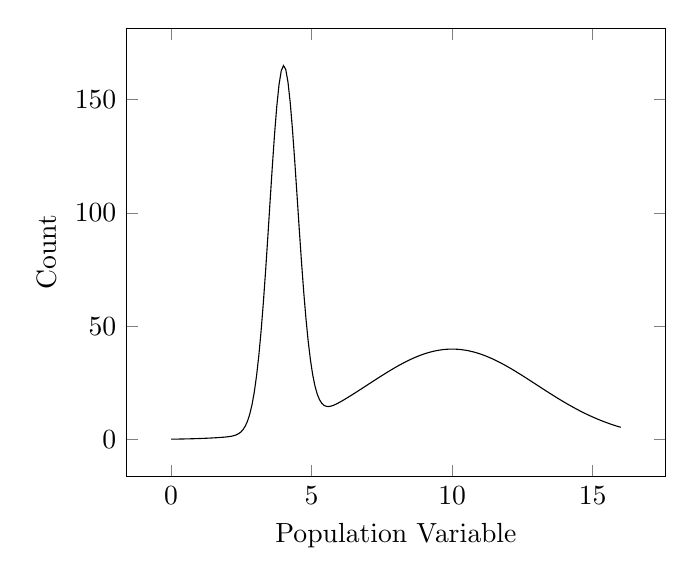
\begin{tikzpicture}
    \begin{axis}[
        ylabel=Count,
        xlabel=Population Variable,
      ]
      \addplot [
        domain=0:16,
        samples=201,
      ]
      {200*exp(-(x-4)^2 / (2*(0.5)^2)) / (sqrt(2*pi*(0.5)^2)) + 
      300*exp(-(x-10)^2 / (2*3^2)) / (sqrt(2*pi*3^2)) };
    \end{axis}
  \end{tikzpicture}
\end{frame}

\begin{frame}
  \frametitle{Data}
  \begin{displaymath}
    \begin{array}{l}
      24.3, \quad 
      20.1, \quad 
      25.4, \quad 
      25.1, \quad 
      19.3, \\[1em]
      21.9, \quad 
      22.9, \quad 
      26.7, \quad 
      19.3, \quad 
      24.7, \\[1em]
      25.3, \quad 
      23.8, \quad 
      23.9, \quad 
      24.1, \quad 
      24.9, \\[1em]
      22.0, \quad
      22.1, \quad 
      21.9, \quad 
      24.9, \quad 
      25.1 
    \end{array}
  \end{displaymath} 
\end{frame}

\begin{frame}
  \frametitle{Data}
  \begin{displaymath}
    \begin{array}{l}
      24.3, \quad 
      20.1, \quad 
      25.4, \quad 
      25.1, \quad 
      19.3, \\[1em]
      21.9, \quad 
      22.9, \quad 
      26.7, \quad 
      19.3, \quad 
      24.7, \\[1em]
      25.3, \quad 
      23.8, \quad 
      23.9, \quad 
      24.1, \quad 
      24.9, \\[1em]
      22.0, \quad
      22.1, \quad 
      21.9, \quad 
      24.9, \quad 
      25.1 
    \end{array}
  \end{displaymath} 
  \vspace{0.3cm}
  \begin{equation*}
    \text{Sample Mean} = \bar{x} = 23.385 \hspace{1cm} 
  \end{equation*}
  \vspace{0.3cm}
  \begin{equation*}
    \text{Sample Standard Deviation} = \sigma = 2.116
  \end{equation*}
\end{frame}

\begin{frame}
  \frametitle{Central Limit Theorem}
  \begin{itemize}
    \item[] 
      Under conditions, sampling distribution will be normal.
      \vspace{0.5cm}
    \item[] 
      For small n, no clear outliers. 
      \vspace{0.5cm}
    \item[] 
      For large n, no extreme outliers.
      \vspace{0.5cm}
    \item[] 
      Make adjustments for small samples?
  \end{itemize}
\end{frame}

\begin{frame}
  \frametitle{t-Distributions}
  \centering
  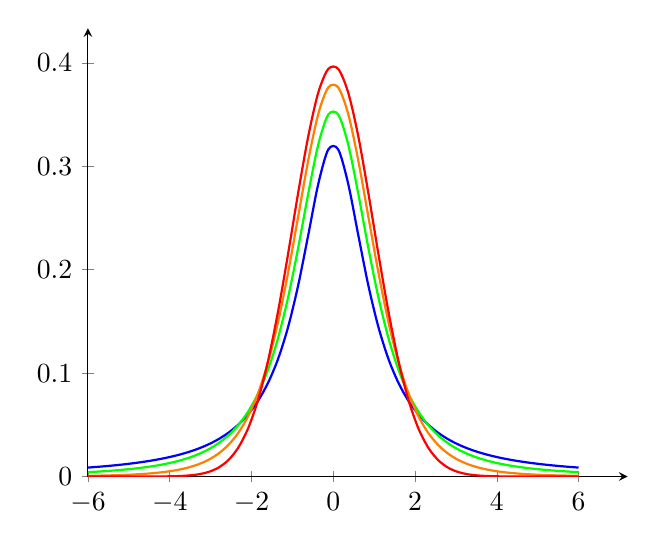
\begin{tikzpicture}[
    declare function={gamma(\z)=
    2.506628274631*sqrt(1/\z)+ 0.20888568*(1/\z)^(1.5)+ 0.00870357*(1/\z)^(2.5)- (174.2106599*(1/\z)^(3.5))/25920- (715.6423511*(1/\z)^(4.5))/1244160)*exp((-ln(1/\z)-1)*\z;},
    declare function={student(\x,\n)= gamma((\n+1)/2.)/(sqrt(\n*pi) *gamma(\n/2.)) *((1+(\x*\x)/\n)^(-(\n+1)/2.));}
]

    \begin{axis}[
      axis lines=left,
      enlargelimits=upper,
      samples=50
      ]
      \addplot [thick, smooth, blue, domain=-6:6] {student(x,1)}; 
      \addplot [thick, smooth, green, domain=-6:6] {student(x,2)}; 
      \addplot [thick, smooth, orange, domain=-6:6] {student(x,5)}; 
      \addplot [thick, smooth, red, domain=-6:6] {student(x,100)}; 
    \end{axis}
  \end{tikzpicture}
  %This code from a stack-exchange question about using tikz to draw
  %the t-distribution
\end{frame}

\begin{frame}
  \frametitle{Hypothesis Testing}
  \begin{itemize}
    \item[] 
      Sample statistic $\bar{x} = 23.385$.
      \vspace{0.2cm}
    \item[] 
      Null hypothesis: population mean $= 21$. 
      \vspace{0.2cm}
    \item[] 
      Alternative hypothesis: population mean $>21$.
      \vspace{0.2cm}
    \item[] 
      Degrees of freedom: $20 - 1 = 19$. 
      \vspace{0.2cm}
    \item[] 
      Standard error: $SE = \frac{\sigma}{\sqrt{n}} =
      \frac{2.116}{\sqrt{20}} = 0.473$
  \end{itemize}
  \vspace{0.4cm}
  \begin{equation*}
    T = \frac{\bar{x} - \text{null value}}{SE} = \frac{23.382 -
    21}{0.473} = 5.036
  \end{equation*}
  \vspace{0.2cm}
  \begin{equation*}
    T = 5.036 \implies p = 0.000367 
  \end{equation*}
\end{frame}

\begin{frame}
  \frametitle{One and Two-Sided Tests}
  \centering
  \begin{tikzpicture}[
    declare function={gamma(\z)=
    2.506628274631*sqrt(1/\z)+ 0.20888568*(1/\z)^(1.5)+ 0.00870357*(1/\z)^(2.5)- (174.2106599*(1/\z)^(3.5))/25920- (715.6423511*(1/\z)^(4.5))/1244160)*exp((-ln(1/\z)-1)*\z;},
    declare function={student(\x,\n)= gamma((\n+1)/2.)/(sqrt(\n*pi) *gamma(\n/2.)) *((1+(\x*\x)/\n)^(-(\n+1)/2.));}
]

    \begin{axis}[
      axis lines=left,
      enlargelimits=upper,
      samples=50
      ]
      \addplot [thick, smooth, blue, domain=-6:6] {student(x,1)}; 
    \end{axis}
  \end{tikzpicture}
  %This code from a stack-exchange question about using tikz to draw
  %the t-distribution
\end{frame}

\begin{frame}
  \frametitle{Confidence Intervals}
  \begin{itemize}
    \item[] 
      Sample statistic $\bar{x} = 23.385$.
      \vspace{0.5cm}
    \item[] 
      Degrees of freedom: $20 - 1 = 19$. 
      \vspace{0.5cm}
    \item[] 
      Standard error: $SE = \frac{\sigma}{\sqrt{n}} =
      \frac{2.116}{\sqrt{20}} = 0.473$
  \end{itemize}
  \vspace{0.4cm}
  \begin{equation*}
    [\bar{x} - (\text{some number})SE, \bar{x} + (\text{some
    number})SE]
  \end{equation*}
  \vspace{0.2cm}
  \begin{equation*}
    [\bar{x} - (2.09)SE, \bar{x} + (2.09)SE] = [22.396, 24.374]
  \end{equation*}
\end{frame}

\end{document}
